\documentclass{beamer}
\usepackage[orientation=portrait,size=a0,scale=1,debug]{beamerposter}
\mode<presentation>{\usetheme{ZH}}
\usepackage[lining]{sourcesanspro}
\usepackage{chemformula}
\usepackage[utf8]{inputenc}
\usepackage[german, english]{babel} % required for rendering German special characters
\usepackage{siunitx} %pretty measurement unit rendering
\usepackage{ragged2e}
\usepackage[font=sourcesanspro,justification=justified]{caption}
\usepackage{array,booktabs,tabularx}
\usepackage{caption}

\usepackage{xcolor}
\usepackage[colorlinks = true, urlcolor  = blue]{hyperref}

\newcommand{\MYhref}[3][blue]{\href{#2}{\color{#1}{#3}}}%


\newcolumntype{Z}{>{\centering\arraybackslash}X} % centered tabularx columns
%\sisetup{per=frac,fraction=sfrac}

\title{\huge Measuring the Geometry of the Universe with the Planck Satellite}
\author{Raul Bermejo$^{1}$}
\institute[UniMelb]{$^{1}$School of Physics, University of Melbourne}
\date{\today}

% edit this depending on how tall your header is. We should make this scaling automatic :-/
\newlength{\columnheight}
\setlength{\columnheight}{104cm}

\begin{document}
\begin{frame}
\begin{columns}
	\begin{column}{.4\textwidth}
		\begin{beamercolorbox}[center]{postercolumn}
			\begin{minipage}{.98\textwidth}  % tweaks the width, makes a new \textwidth
				\parbox[t][\columnheight]{\textwidth}{ % must be some better way to set the the height, width and textwidth simultaneously
					\begin{myblock}{Introduction}	The Cosmic Microwave Background (CMB) is the first electromagnetic signal we can study after the Big Bang. It thus encodes a wealth of cosmological information from the epoch of recombination (and reionization). In this study, we use data from the Planck satellite mission to measure the anisotropy of the CMB. Studying the statistical fluctuations in this primordial signal allows us to infer the geometry of the Universe.

%\vspace{0.4em}
%\begin{figure}
%\begin{minipage}{0.43\textwidth}
%	\centering\includegraphics[width=0.85\textwidth]{poster_labyCMB/img/PlanckCMB_commander.png}
%	\caption{CMB as measured by the Planck satellite \cite{planck:2018_iv}.}
%	\label{fig:esa_cmb}
%\end{minipage}
%\hspace{1em} 
%\end{figure}

\vspace{0.5em}
\begin{figure}
	\begin{minipage}{0.3\textwidth}
		\centering\includegraphics[width=1.1\textwidth]{poster_labyCMB/img/sphere.png}
	\end{minipage}
	\hspace{1em}
	\begin{minipage}{0.3\textwidth}
	    \captionsetup{width=2\textwidth}
		\centering\includegraphics[width=1\textwidth]{poster_labyCMB/img/flat.png}
		\hspace{14em}\caption{Different geometries that the universe can take. From left to right: positively curved (closed $k=1$), no curvature (flat $k=0$) and negatively curved (open $k=-1$).}
		\label{fig:geometries}
	\end{minipage}
	\hspace{1em}
	\begin{minipage}{0.3\textwidth} 
		\centering\includegraphics[width=1\textwidth]{poster_labyCMB/img/saddle.png}
	\end{minipage}
\end{figure}

In the standard $\Lambda$CDM model of cosmology [add reference?], the geometry of the Universe is encoded in the \textit{curvature density parameter}, $\Omega_k$:

\begin{equation}
    \Omega_{k}=-\frac{k c^{2}}{a^{2} H^{2}},
\end{equation}
\hspace{1em} 

where $k$ corresponds to the curvature of the Universe, $c$ is the speed of light, $a$ is the expansion scale factor, and $H = \frac{\dot{a}}{a}$ is the Hubble-Lemaître parameter. $\Omega_k$ indicates the energy contribution to the Universe due to its curvature, and $k = −1, +1, 0$ corresponds to an open, closed or flat Universe respectively, as shown in figure ~\ref{fig:geometries}.

By comparing the CMB signal from that of simulated Universes with different values of $\Omega_k$ (also known as Boltzmann codes, see \cite{lesgourgues:2011}), we can infer the value of $\Omega_k$ corresponding to our Universe. 
				
						
					\end{myblock}\vfill
					
					
					\begin{myblock}{Planck Dataset}
					We study Lorem ipsum dolor sit amet, consectetur adipiscing elit. Nullam porta ornare ligula, at accumsan elit commodo et. Curabitur sagittis risus augue, eleifend porta nunc hendrerit vitae. Ut ipsum nisl, finibus in euismod id, ullamcorper vel lorem. Proin ut velit ut orci sagittis dapibus sed ac lectus. Vestibulum at vulputate lectus. Etiam fermentum mi ex, quis bibendum ex euismod laoreet. Quisque nunc augue, porta quis efficitur vel, porttitor eget tellus ~\ref{fig:tt}.

\vspace{0.5em}
\begin{figure}
	\begin{minipage}{0.94\textwidth}
		\centering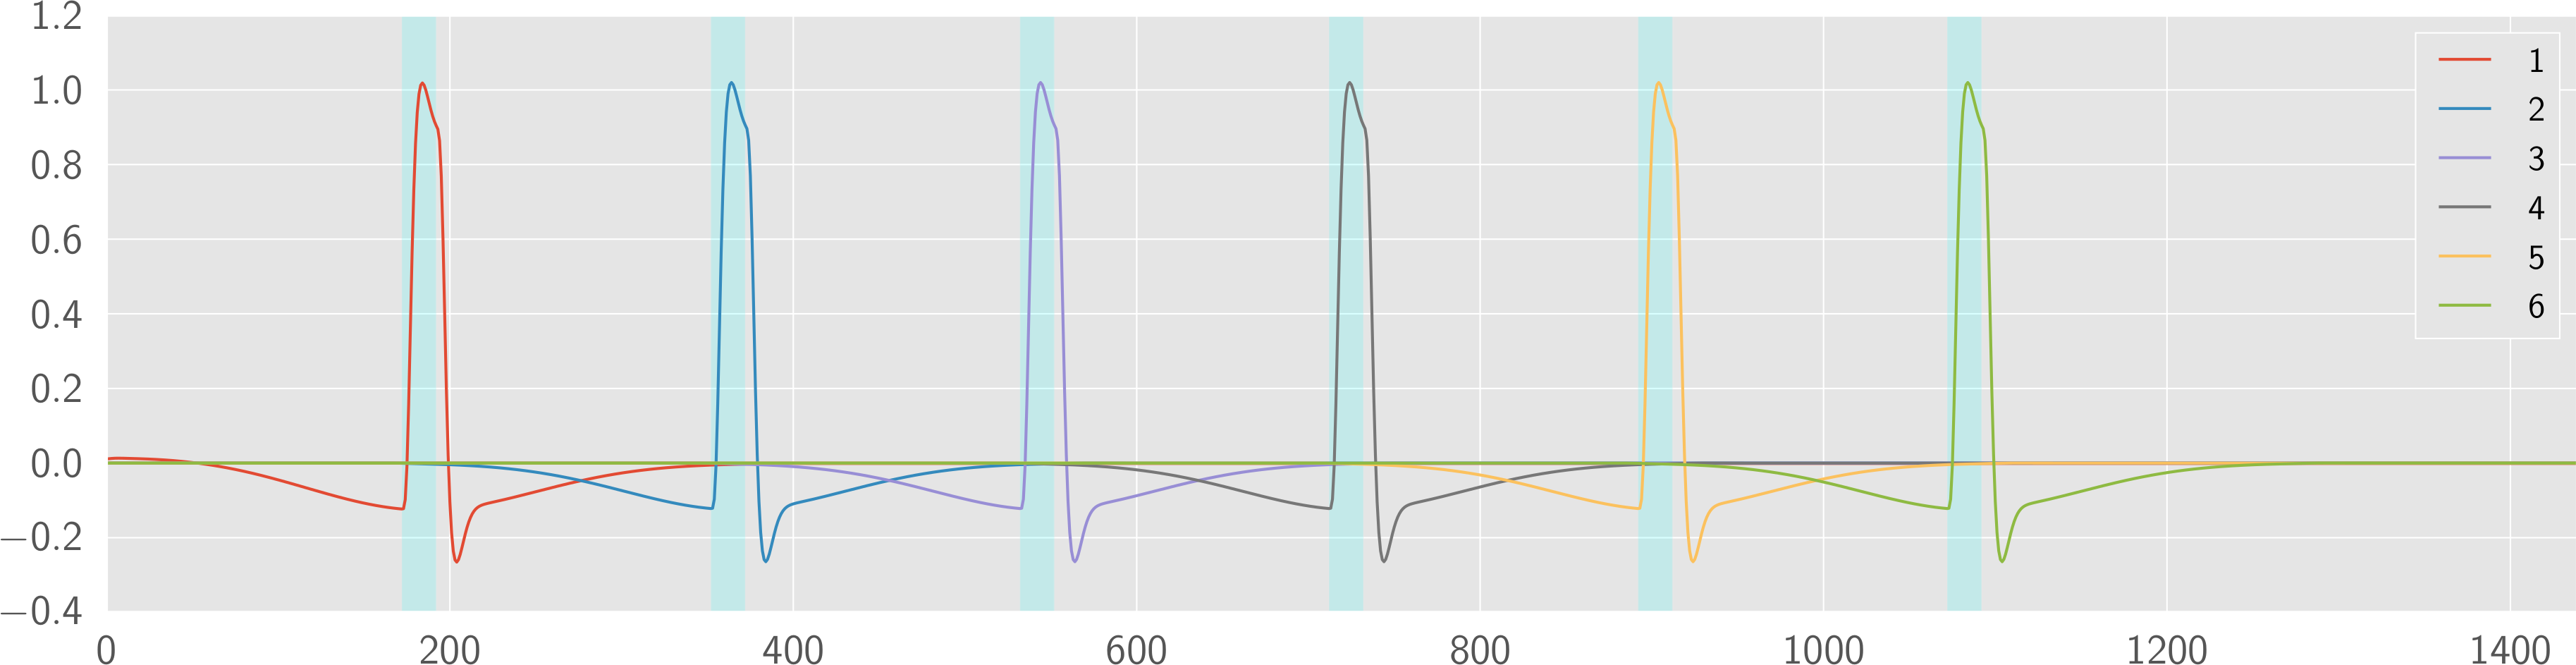
\includegraphics[width=0.9\textwidth]{img/dm.png}
		\caption{Ut ipsum nisl.}
		\label{fig:stim}
	\end{minipage}
\end{figure}

\begin{itemize}

	\item filter 1 (as seen in figure~\ref{fig:stim}).
	
 	\item filter 2 (as seen in figure~\ref{fig:stim}).
 	
 	\item filter 3 (as seen in figure~\ref{fig:stim}).
 	
\end{itemize}
\vspace{0.5em}
\begin{figure}
	\begin{minipage}{0.94\textwidth}
		\centering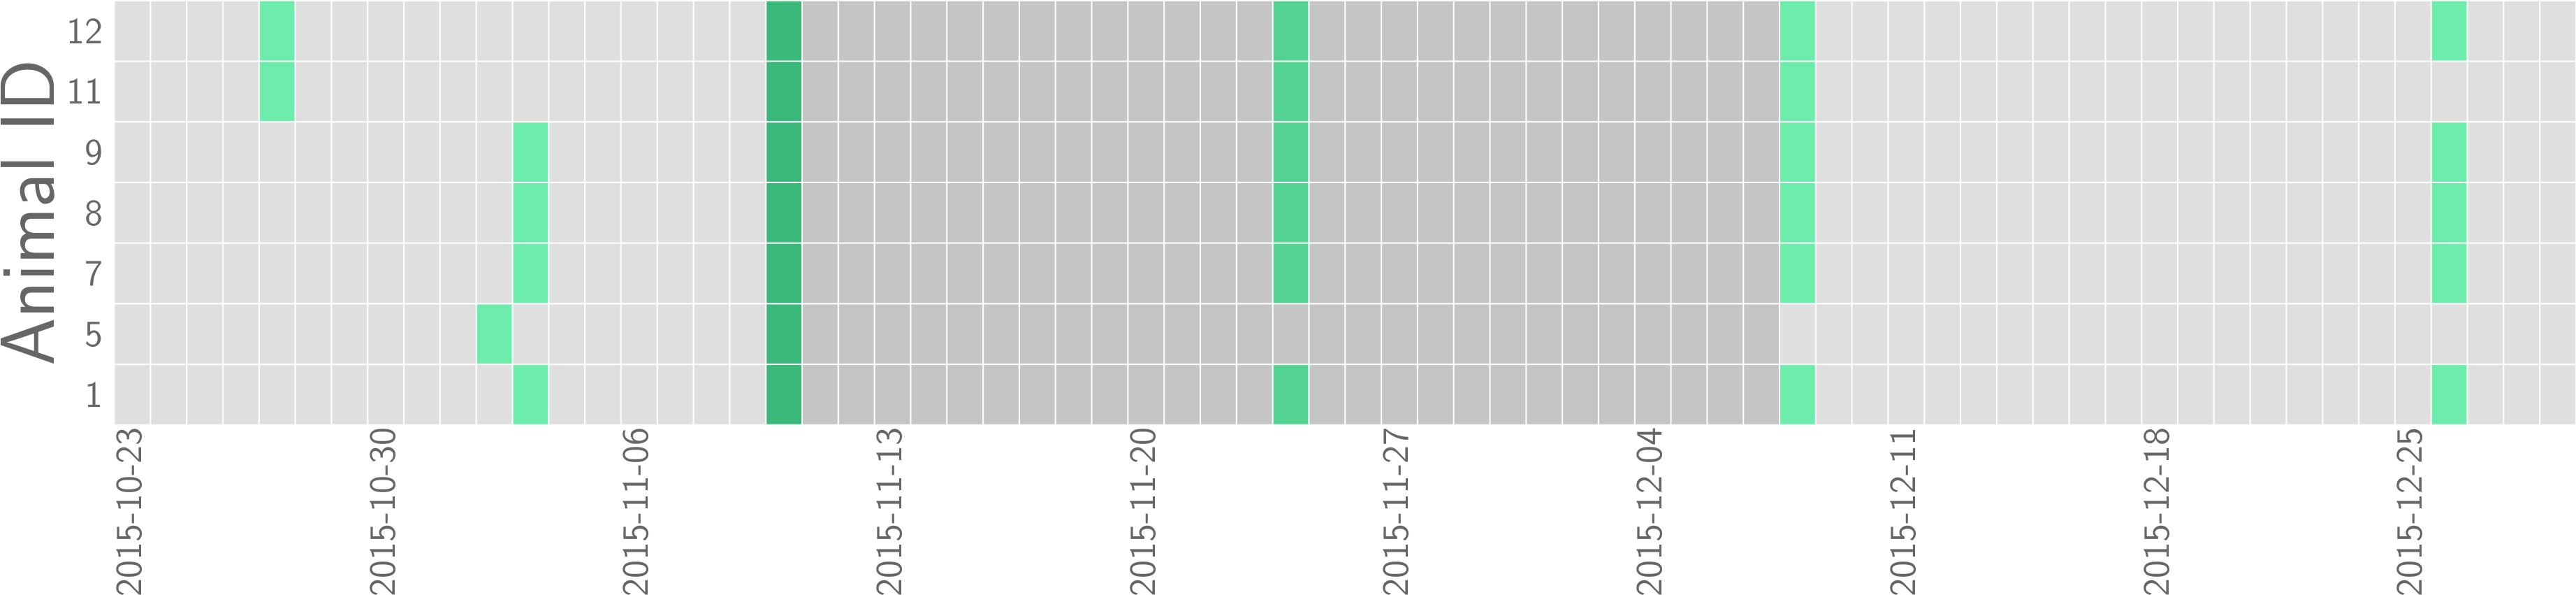
\includegraphics[width=0.9\textwidth]{img/tt.png}
		\caption{quis bibendum ex euismod laoreet}
		\label{fig:tt}
	\end{minipage}
\end{figure}
					\end{myblock}\vfill
		}\end{minipage}\end{beamercolorbox}
	\end{column}
	
	
	\begin{column}{.6\textwidth}
		\begin{beamercolorbox}[center]{postercolumn}
			\begin{minipage}{.98\textwidth} % tweaks the width, makes a new \textwidth
				\parbox[t][\columnheight]{\textwidth}{ % must be some better way to set the the height, width and textwidth simultaneously
					\begin{myblock}{Cross Power Spectrum}
					
					We infer the geometrical signal from the Planck data by studying the fluctuations in temperature $\Delta T$ from the Planck sky maps. These fluctuations in the signal can be described by the so-called \textit{cross power spectrum} $C_{\ell}$. An unbiased estimator for $C_{\ell}$ \cite{tristram:2005} is given by 

\begin{equation}
\widehat{C_{\ell}}=\sum_{m=-\ell}^{\ell} \frac{\left|a_{\ell m}\right|^{2}}{2 \ell+1},
\end{equation}
\vspace{1em}

where $\ell$ corresponds to the multipole (associated with an angular size) and $a_{\ell}$ corresponds to the Fourier coefficients of the spherical harmonic decomposition of $\Delta T$:

\begin{equation}
a_{\ell m}=\int \Delta T(\hat{n}) Y_{\ell m}(\hat{n}) d \Omega.
\end{equation}
\vspace{1em}

We compute $C_{\ell}$ using the open-source Python package \textsc{healpy} (\cite{healpy:2019}; \cite{healpix:2005}). Next, to reduce the correlations and errors in $C_{\ell}$ induced by the cut sky, we bin the cross power spectrum. Following \cite{hivon:2002}, we choose the 'flattened spectrum' as our binning such that $C_{\ell} \equiv \ell(\ell+1) C_{\ell} / 2 \pi$.


\vspace{0.8em}
\begin{figure}
	\begin{minipage}{.65\textwidth}
		\centering\includegraphics[width=.85\textwidth]{poster_labyCMB/img/BoltzCode_Cls.png}
		\caption{Cross power spectra for simulated Universes with different $\Omega_k$.}
		\label{fig: boltz_Cls}
	\end{minipage}
\end{figure}
\vspace{0.8em}

The first peak of $C_l$ encodes the information about $\Omega_k$ [add reference!]. From figure ~\ref{fig: boltz_Cls}, one can see that different values of $\Omega_k$ shift the value of $\ell_{peak}$ along the x-axis.

Thus to infer $\Omega_k$, we fit the value $\ell_{peak}$ from the Planck sky maps to that of a set of simulated Universes with different values of $\Omega_k$ (and thus different geometries). These simulated power spectra were computed by using the Boltzmann Code Python package \textsc{CAMB} \cite{camb:2011}.

					\end{myblock}\vfill
					
					
					\begin{myblock}{Results}
					\begin{figure}
	\begin{minipage}{0.95\textwidth}
		\centering\includegraphics[width=0.85\textwidth]{poster_labyCMB/img/Planck_Cl_143x143__60perc.png}
		\caption{Computed cross-power spectrum from the Planck satellite.}
		\label{fig:planck_cls}
	\end{minipage}
\end{figure}

As we are only interested in the first peak of the cross power spectrum, we fitted the computed $C_{\ell}$ for the Planck data using the following model:

\begin{equation}
    C_{\ell} = a(\ell-\ell_{peak})^2 + b,
\end{equation}

where $a, \ell_{peak}$ and $b$ are model parameters. Figure \ref{fig:planck_cl} shows the fit for the model, with a multipole value of $\ell_{peak} = 211.14 \pm 1.10$.

Finally, using the curves in figure \ref{fig: boltz_Cls} and our estimated $\ell_{peak}$, we performed a one-dimensional fit to find an estimate of $\Omega_k$. Our estimate of the curvature density parameter as measured by the Planck satellite data corresponds to 

\begin{equation*}
    \Omega_k = -0.028 \pm 0.012.
\end{equation*}

This result is within a $2\sigma$ accordance with respect to literature values from the Planck 2018 release \cite{planck:2018_main}, thus suggesting a flat geometry for our Universe. 

	

					\end{myblock}\vfill
					
					
					
					\begin{myblock}{References}
						\footnotesize
						\bibliographystyle{abbrv}
						\bibliography{references}
					\end{myblock}\vfill
		}\end{minipage}\end{beamercolorbox}
	\end{column}
\end{columns}
\end{frame}
\end{document}
